\section{Results}

\begin{figure*}[t]
\centering
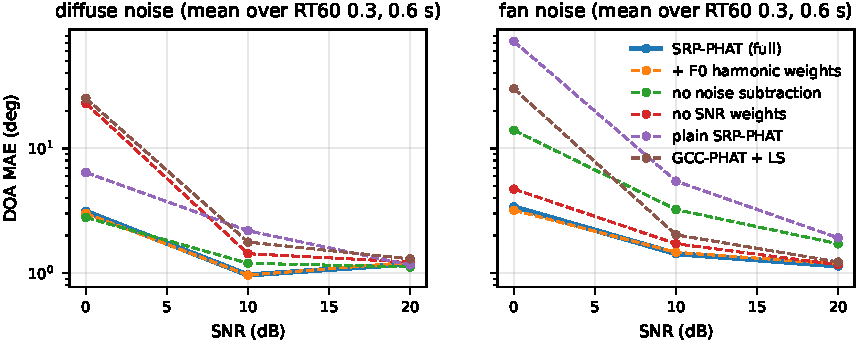
\includegraphics[width=\textwidth]{figures/doa_error.pdf}
\caption{DOA mean absolute error (log scale) versus SNR, averaged over
RT$_{60}$ 0.3 and 0.6\,s, talker at 1.5\,m. Removing either use of the
silence model hurts in one noise condition; removing both fails with a
directional noise source.}
\label{fig:doa}
\end{figure*}

\paragraph{Angle.} Figure~\ref{fig:doa}. At 20\,dB SNR all estimators are
within about $2^\circ$. At 0\,dB the two uses of the silence model matter in
different conditions. With diffuse noise, dropping the speech-presence
weights raises the error from \doadiffusesrpsnrZerortThree/\doadiffusesrpsnrZerortSix$^\circ$
(RT$_{60}$ 0.3/0.6\,s) to
\doadiffusesrpnosnrwsnrZerortThree/\doadiffusesrpnosnrwsnrZerortSix$^\circ$:
after subtraction, noise-only bins carry structured residue that PHAT
normalises to full weight. With the fan, dropping the subtraction raises it
from \doafansrpsnrZerortThree/\doafansrpsnrZerortSix$^\circ$ to
\doafansrpnonsubsnrZerortThree/\doafansrpnonsubsnrZerortSix$^\circ$, and
plain SRP-PHAT locks on the fan
(\doafansrpplainsnrZerortThree/\doafansrpplainsnrZerortSix$^\circ$).
GCC-PHAT with least squares reaches
\doadiffusegccsnrZerortThree--\doafangccsnrZerortSix$^\circ$ at 0\,dB. The
$F_0$-harmonic comb changes nothing measurable on our synthetic talker,
whose spectrum is already purely harmonic.

\begin{figure}[t]
\centering
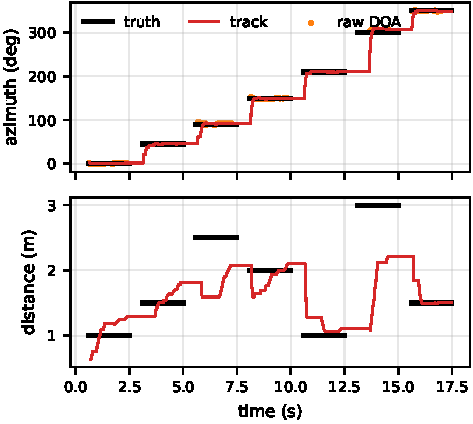
\includegraphics[width=\linewidth]{figures/radar_demo_track.pdf}
\caption{Streaming estimates for a talker moving through 7 positions
(black: truth). Top: azimuth. Bottom: distance.}
\label{fig:demo}
\end{figure}

\paragraph{Tracking a moving talker.} Figure~\ref{fig:demo}: after
0.5\,s of settling per position, the tracked azimuth has a median error of
\demoAzMedErr$^\circ$ (90th percentile \demoAzPNinetyErr$^\circ$). The
distance track (model trained in the same room) has a median error of
\demoRangeMedErr\,m and under-estimates the 3\,m position.

\begin{figure*}[t]
\centering
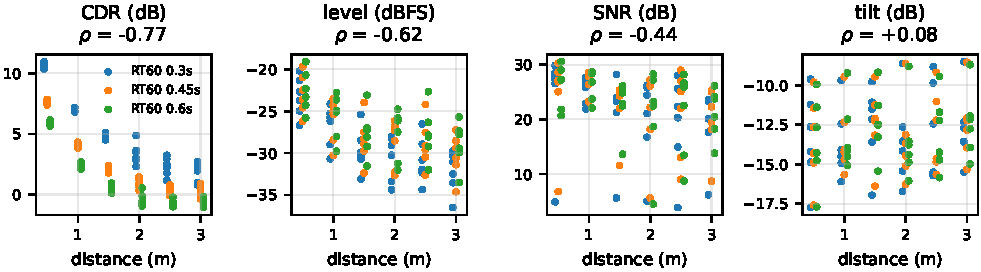
\includegraphics[width=\textwidth]{figures/distance_features.pdf}
\caption{Distance features versus true distance (\distN{} clips), coloured
by RT$_{60}$; $\rho$ is Spearman's correlation with $\log r$ over all
rooms. CDR is monotone within each room but offset between rooms.}
\label{fig:distfeat}
\end{figure*}

\begin{figure}[t]
\centering
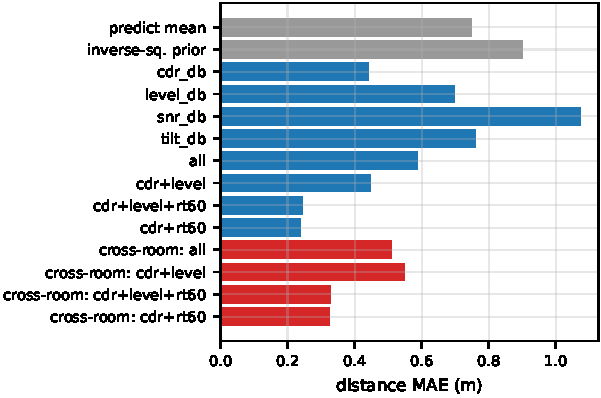
\includegraphics[width=\linewidth]{figures/distance_cv.pdf}
\caption{Distance MAE. Blue: leave-one-angle-out; red: leave-one-RT$_{60}$-out.}
\label{fig:distcv}
\end{figure}

\paragraph{Distance.} Figure~\ref{fig:distfeat}: the CDR is the strongest
cue ($\rho=\rhocdrdb$ pooled, \rhoCdrRoomMax{} to \rhoCdrRoomMin{} within a room). Level
($\rho=\rholeveldb$) suffers from the $\pm$4\,dB vocal-effort jitter, SNR
($\rhosnrdb$) from how much speech leaks into the noise estimate, and tilt
($\rhotiltdb$) carries little information. Figure~\ref{fig:distcv}: across
angles, CDR alone gives \distcvcdrdb\,m MAE and CDR + level
\distcvcdrlevel\,m, against \distPredictMean\,m for predicting the mean and
\distPrior\,m for an inverse-square law on level. Adding the room's
RT$_{60}$ gives \distcvcdrrtSixZero\,m, and across rooms (leave one
RT$_{60}$ out) \distxroomcdrrtSixZero\,m versus \distxroomcdrlevel\,m
without it.

\begin{figure}[t]
\centering
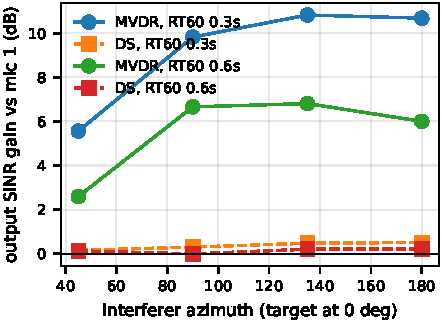
\includegraphics[width=\linewidth]{figures/beamform_gain.pdf}
\caption{Output SINR gain over microphone 1 against a competing talker
(target at $0^\circ$, both at 1.2\,m, SIR 0\,dB), with steering from the
estimated DOA.}
\label{fig:beam}
\end{figure}

\paragraph{Selective cancellation.} Figure~\ref{fig:beam}: MVDR gains
\beamMvdrMin--\beamMvdrMax\,dB (mean \beamMvdrMean\,dB), less in the more
reverberant room and at $45^\circ$ separation, where the estimated target
DOA was also furthest off (\beamDoaErrMax$^\circ$). Delay-and-sum gains
\beamDsMean\,dB: at 1\,kHz the array spans 0.19 wavelengths, so only
superdirective weights give selectivity.
